\documentclass[tikz,border=10pt]{standalone}
\usepackage{amsmath}
\begin{document}
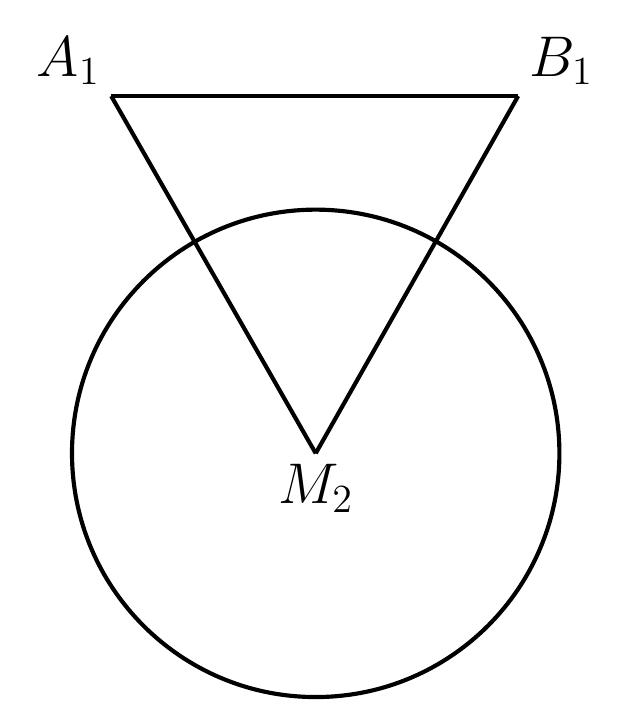
\begin{tikzpicture}[line width=1.5pt, line join=round]
  % Scale: 1 px = 0.02623 cm, origin at M2 (apex and circle centre)
  \coordinate (M) at (0,0);
  \coordinate (A) at (-2.597,4.538);   % A1 = (79,48) px
  \coordinate (B) at (2.571,4.538);    % B1 = (276,48) px

  % Top side and the two sides meeting at the apex
  \draw (A) -- (B);
  \draw (A) -- (M);
  \draw (B) -- (M);

  % Full circle centred at M2, radius 118 px
  \draw (M) circle (3.095);

  % Labels
  \node[font=\fontsize{21}{25.2}\selectfont, above left] at (A) {$A_1$};
  \node[font=\fontsize{21}{25.2}\selectfont, above right] at (B) {$B_1$};
  \node[font=\fontsize{21}{25.2}\selectfont, below] at (M) {$M_2$};
\end{tikzpicture}
\end{document}